\section{Background}

FHIR (Fast Health Interoperability Resources) is a standard to exchange healthcare information electronically  \cite{FHIRClinician}. FHIR offers a strong focus on  implementability in a wide variety of architectures and scenarios \cite{FHIRExecutive}. The current version of FHIR is Release 4 \cite{FHIR}.

OpenEHR is a platform focus for the development of information technology solutions for healthcare. OpenEHR provides a set of standards for models of clinical information, EHR extracts, demographic data, types of data and several types of service interfaces \cite{openEHRWhitePaper}.

\subsection{FHIR}

FHIR define recursos para representar conceptos administrativos tales como paciente, proveedor, organización y dispositivo, así como conceptos clínicos que cubren problemas, medicamentos, diagnósticos, planes de atención y más \cite{FHIRResourceList}.

Los recursos tienen en común las siguientes características \cite{FHIRDeveloper}:
\begin{itemize}
  \item una URL que identifica el recurso;
  \item una metainformación común;
  \item un texto legible por el ser humano para la seguridad clínica;
  \item un conjunto definido de elementos de datos diferente para cada recurso;
  \item un marco para extender y adaptar los recursos existentes.
\end{itemize}

Los recursos se describen usando recursos StructureDefinition \cite{FHIRStructureDefinition}. Estos recursos StructureDefinition definen un conjunto de elementos de datos. Cada elemento incluye una ruta, una cardinalidad y un tipo de dato \cite{FHIRElementDefinition}.

La ruta del elemento de dato es la propiedad más importante de la definición del elemento. Esta ruta localiza el elemento en una jerarquía definida dentro del recurso \cite{FHIRElementDefinition}.

El tipo de dato del elemento de dato puede ser primitivo o complejo \cite{FHIRDataTypes}. La diferencia entre ambos tipos de datos es que el primitivo permite un solo valor para el elemento,  mientras que el complejo puede tener elementos hijos. Cada tipo de dato primitivo es una 3-tupla, que consiste en a) un dominio de valores, que incluye la definición del tipo de dato, b) una representación XML y c) una representación JSON. Dentro de los tipos de datos complejos se encuentran: los de propósito general, los tipos para metadatos y los de propósito especial.

Cada elemento de dato puede ser extendido o restringido \cite{FHIRProfiling}. El elemento de dato se extiende para representar información adicional que no forma parte de la definición del recurso\cite{FHIRExtensibility}. Cada recurso solo incluye elementos de datos si la mayoría de las implementaciones usarán esos elementos de datos en particular \cite{FHIRArchitecture}. El elemento de dato se restringe cambiando su cardinalidad.

Los recursos soportan la vinculación a terminología clínica, lo cual contribuye al uso de FHIR para lograr la interoperabilidad semántica \cite{FHIRArchitecture}.

Aparte de las definiciones de los recursos, FHIR define un conjunto de interfaces por las cuales los sistemas comparten los recursos. Los mecanismos de intercambio soportados son los siguientes \cite{FHIRClinician}:
\begin{itemize}
  \item a través de una interfaz REST;
  \item mediante el intercambio de documentos;
  \item vía el envío y recepción de mensajes;
  \item la exposición e invocación de servicios.
\end{itemize}


\subsection{openEHR}

El enfoque de openEHR es un riguroso modelado del conocimiento, y se basa en el principio básico de separación de los dominios de concepto y los dominios de información en los sistemas de información. Los dominios de concepto son modelados usando los arquetipos y expresados en el Lenguaje de Definición de Arquetipos (ADL). Estos conceptos son profundizados a continuación.

\subsubsection{Modelado en openEHR}

El enfoque de openEHR para el modelado es multinivel. Los modelos son desarrollados y mantenidos por expertos de dominio en su propio nivel \cite{openEHRArchitecture}.

El primer nivel se basa en el modelo de referencia. El modelo de referencia corresponde al modelo de información estable, por ejemplo, tipos de datos o estructuras de datos. Todos los datos EHR en cualquier sistema openEHR obedecen el modelo de referencia. Solo este primer nivel es implementado en software \cite{openEHRArchitecture}.

El siguiente nivel consiste en los arquetipos. Los arquetipos corresponden a los contenidos del dominio, por ejemplo, medidas de la presión sanguínea o resultado de la prueba para diabetes. Estos arquetipos son modelados por profesionales clínicos o expertos en informática de la salud sin ningún conocimiento tecnológico de los sistemas finales. Los arquetipos son almacenados en sus propios repositorios.

Las plantillas constituyen el siguiente nivel. Estas plantillas especifican grupos de arquetipos que se usan para un propósito particular, y a menudo corresponden a formularios de pantalla \cite{openEHRArchitecture}.

En el último nivel se encuentran los artefactos generados a partir de las plantillas. Estos artefactos pueden ser interfaces de programas, XSDs, componentes de interfaces de usuarios \cite{openEHR}.

La Figura \ref{fig:openeEHR_ecosystem} ilustra el modelado multinivel.

\begin{figure}[h]
  \centering
  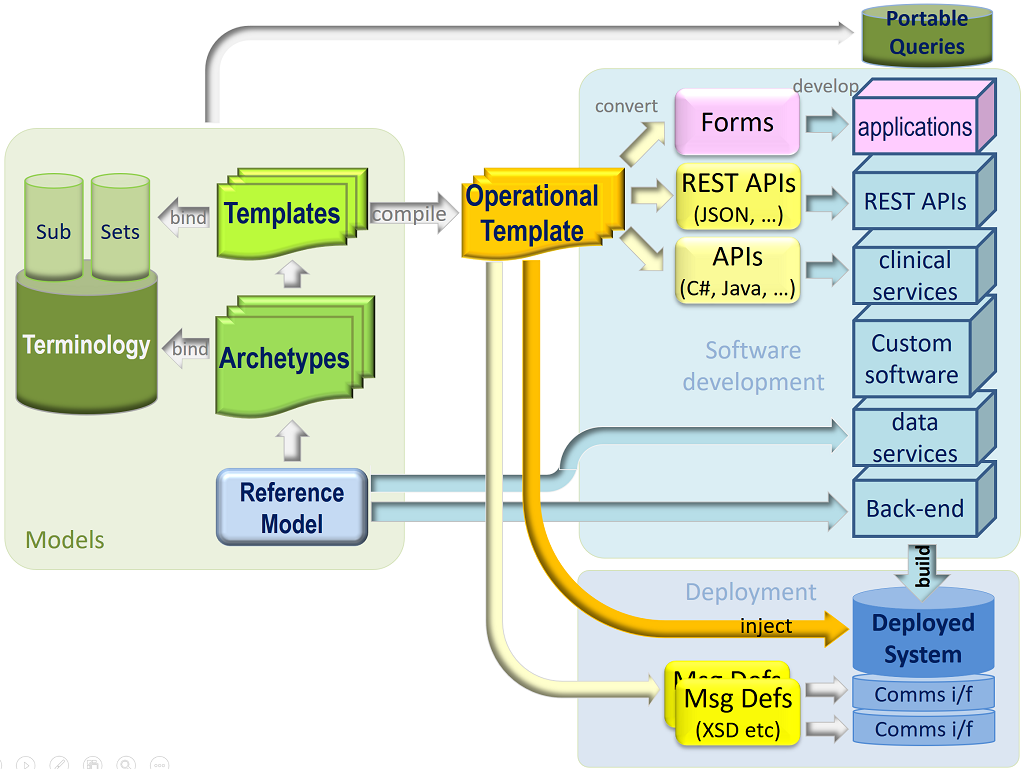
\includegraphics[scale=0.6]{./images/openehr_dev_ecosystem}
  \caption{Enfoque openEHR}
  \label{fig:openeEHR_ecosystem}
\end{figure}


\subsubsection{Arquetipos}

Cada arquetipo es un conjunto de restricciones en el modelo de referencia, definiendo un contenido de dominio \cite{openEHRArchitecture}. Las restricciones definen configuraciones de instancias del modelo de referencia consideradas conformes al arquetipo. Por ejemplo, ciertas configuraciones de las clases PARTY, ADDRESS, CLUSTER y ELEMENT pueden definirse por un arquetipo Person como estructuras permitidas para personas con identidad, contactos y direcciones \cite{openEHRAOM}.

Los arquetipos pueden tener relaciones de especialización y/o composición. Los arquetipos especializados son creados restringiendo aún más las restricciones existentes de otros arquetipos. Los arquetipos compuestos son definidos a partir de otros arquetipos \cite{openEHRArchitecture}.

OpenEHR incluye un mecanismo de rutas. Estas rutas pueden usarse para referenciar a cualquier dato dentro de un arquetipo \cite{openEHRArchitecture}.

Los arquetipos proveen una forma de definir el significado de los datos, y de conectar los datos a terminologías conocidas como SNOMED CT, LOINC, ICPC, ICDx y muchas otras terminologías y vocabularios usados en salud \cite{openEHRArchitecture}.


\subsubsection{Lenguaje de Definición de Arquetipo}

Los arquetipos son expresados en el Lenguaje de Definición de Arquetipo \cite{openEHRADL} (ADL por sus siglas en inglés). ADL utiliza tres sintaxis: cADL (forma de restricción de ADL), ODIN (notación de instancia de datos de objeto) y una versión de lógica de predicado de primer orden (FOPL por sus siglas en inglés).

Las restricciones de cADL se escriben en un estilo estructurado en bloques, similar a los lenguajes de programación estructurados en bloques como C. Cada bloque se introduce mediante un identificador de un modelo de información de openEHR. Los identificadores alternan entre los nombres de tipo conocidos como bloques de objetos o nodos de objeto y los nombres de atributos de tipo conocidos como bloques de atributo o nodos de atributos. El uso de nodos de objeto permite la formación de rutas de arquetipo, que se pueden utilizar para hacer de forma inequívoca a nodos de objetos dentro del mismo arquetipo \cite{openEHRADL}.

La sintaxis de cADL se utiliza para expresar la definición de los arquetipos, mientras que la sintaxis de ODIN se usa para expresar datos que aparecen en las secciones de idioma, descripción, terminología y revisión histórica de un arquetipo.

Actualmente hay dos versiones principales existentes: `ADL 1.4', la versión original, y `ADL 2', una versión más moderna, que se está adoptando lentamente.



\subsection{Arquitectura de conversión de datos}

La arquitectura del Modelo de Información de Integración de openEHR, mostrado en la Figura \ref{fig:data_conversion_architecture}, está diseñado para situaciones de integración heredadas.

\begin{figure}[h]
  \centering
  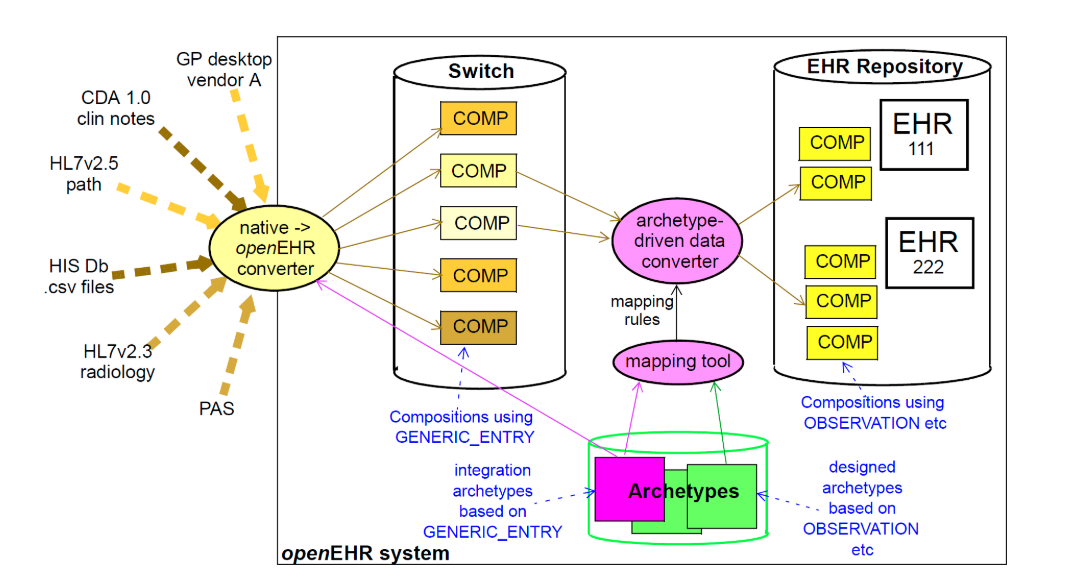
\includegraphics[scale=0.4]{./images/data_conversion_architecture}
  \caption{Integración de dato dentro de openEHR (Fuente: Extraído desde \cite{openEHR}).}
  \label{fig:data_conversion_architecture}
\end{figure}

La base del diseño se basa en una clara separación de la transformación sintáctica y semántica requerida en los datos importados en openEHR. La transformación sintáctica convierte los datos de su formato sintáctico original en estructuras del modelo de referencia de openEHR, cuya estructura lógica y semántica está controladas por arquetipos de integración que imitan el diseño original de los datos. Como resultado de la conversión, los datos son susceptibles de ser procesados en openEHR. La transformación semántica convierte los datos importados a arquetipos clínicos.

Los elementos de openEHR que hacen posible esta transformación son:
\begin{itemize}
  \item la clase GENERIC\_ENTRY que se utiliza para crear representaciones intermedias de datos de fuentes que de otra manera no se ajustan a las clases openEHR;
  \item arquetipos de integración definidos en contra de la clase GENERIC\_ENTRY;
  \item reglas de transformación semántica de los datos de openEHR basados en GENERIC\_ENTRY y arquetipos de integración a los datos basados en los subtipos de ENTRY, y arquetipos clínicos diseñados.
\end{itemize}


FHIR and openEHR share certain similarities. FHIR resources and openEHR archetypes define reusable patterns for the precise description of clinical information \cite{Bosca15}. Nevertheless, collaboration works between FHIR and openEHR communities \cite{Collaboration} could not generate resources and archetypes with matching and clinically verifiable content. One of the causes for this is different design principles utilized by both communities. The main difference being that the archetypes are expected to represent the majority of the clinical content, while the resources only contain the most common clinical information used.

The approach proposed in this work uses the StructureDefinition FHIR resources to create openEHR integration archetypes using classes CLUSTER and ELEMENT. These integration archetypes, expressed in ADL, will facilitate the data exchange between FHIR and openEHR systems. The exchange is accomplished by establishing mappings between the paths of resource elements and the paths of archetype node. Different from GENERIC\_ENTRY class, which makes no assumptions about the real form of the data, classes CLUSTER and ELEMENT represent the hierarchal structure of FHIR resources. Besides, the proposed approach uses the binding connections between information models and terminologies, supported by both standards to conserve the meaning of the exchanged data.
